\documentclass[11pt]{article}

\usepackage[margin=1in]{geometry}
\usepackage{graphicx}
\usepackage{hyperref}
\usepackage{xcolor}
\usepackage{listings}
\usepackage{cite}

\lstset{
  basicstyle=\ttfamily\small,
  breaklines=true,
  columns=fullflexible,
  frame=single,
  rulecolor=\color{black!20},
  keywordstyle=\color{blue!60!black},
  commentstyle=\color{black!60},
  stringstyle=\color{green!40!black},
  showstringspaces=false
}

\title{COMP7940 Cloud Computing\\Lab 6: Chatbot in Docker}
\author{
  Name: ZHAO Zhan \\
  Student ID: 25482351 \\
  GitHub: @Extious
}
\date{\today}

\begin{document}
\maketitle

\section*{1. Docker Image and Container Workflow}

The chatbot was containerized using a \texttt{Dockerfile} based on \texttt{python:3.12-slim}.
Dependencies are installed from \texttt{requirements.txt}, and only the Python modules \texttt{chatbot.py} and \texttt{ChatGPT\_HKBU.py} are copied into the image.
Runtime credentials are \emph{not} baked into the image; instead, \texttt{config.ini} is supplied at container startup by bind-mounting a host file into \texttt{/comp7940-lab/config.ini}.
The image was built with:

\begin{lstlisting}[language=bash]
docker build -t lab6-chatbot .
\end{lstlisting}

The container was started in detached mode with a volume mount so the bot reads the local configuration file inside the container:

\begin{lstlisting}[language=bash]
docker run -d --name chatbot-container \
  -v /absolute/path/to/config.ini:/comp7940-lab/config.ini \
  lab6-chatbot
\end{lstlisting}

The lab instructions use the image name \texttt{chatbot}; the same workflow applies after tagging the image as \texttt{chatbot} with \texttt{docker build -t chatbot .}.

\section*{2. Container Logs}

Figure~\ref{fig:docker-logs} shows \texttt{docker logs chatbot-container} output after a successful startup: configuration is loaded, the Telegram application is initialized, message handling is registered, and polling begins.

\begin{figure}[htbp]
  \centering
  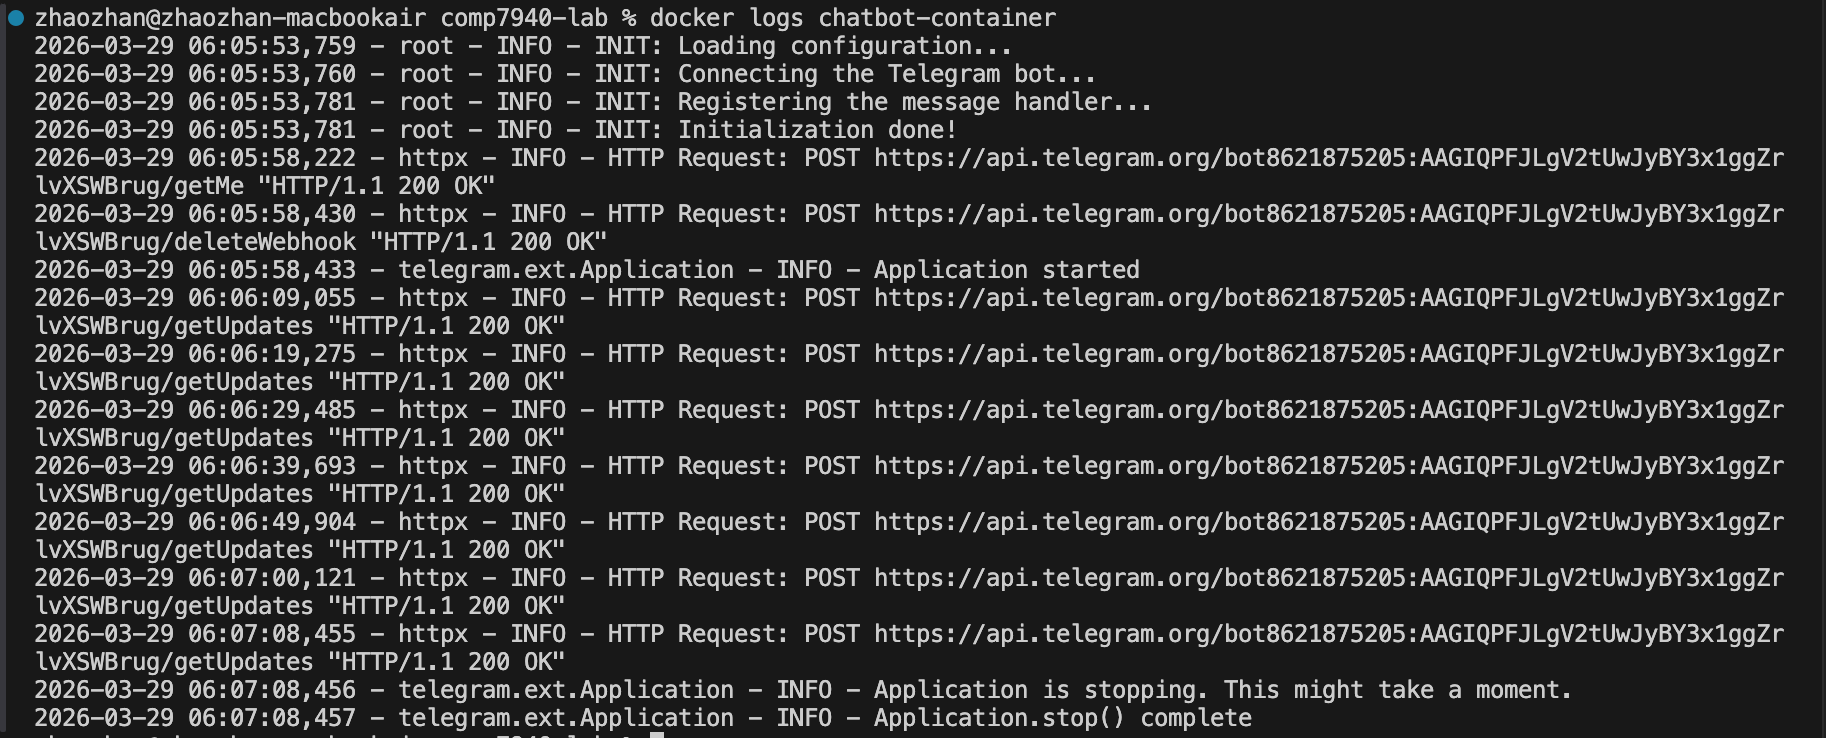
\includegraphics[width=0.95\linewidth]{lab6/logs.png}
  \caption{Docker logs for \texttt{chatbot-container}, showing initialization and Telegram polling.}
  \label{fig:docker-logs}
\end{figure}

\section*{3. Write-Up Questions}

\subsection*{Q1: Explain why a Docker image should not contain \texttt{config.ini}}

Including \texttt{config.ini} in the image is discouraged when that file holds secrets (Telegram bot token, API keys, endpoints) or environment-specific settings:

\begin{enumerate}
  \item \textbf{Secrets become part of image layers.}
    Anything \texttt{COPY}ed into an image is stored in the image filesystem and its layers.
    Anyone who can \texttt{docker pull} the image, receive a \texttt{.tar} export, or access a registry can extract files from those layers and recover the credentials~\cite{docker-docs}.

  \item \textbf{History and sharing.}
    Image layers persist in build cache and registries; accidentally pushing an image that embeds secrets leaks them broadly and permanently unless layers are fully discarded.
    Re-tagging or rebuilding does not remove secrets already published in an old layer.

  \item \textbf{Separation of code and configuration.}
    The same image should be able to run in development, staging, or production with different tokens and URLs.
    Twelve-factor style guidance treats config as environment-specific data supplied at runtime (files, environment variables, or secret stores), not baked into the build artifact~\cite{twelve-factor-config}.

  \item \textbf{Operational rotation.}
    If a token is rotated, mounting \texttt{config.ini} or injecting env vars avoids rebuilding and redeploying the image solely to change secrets; only the runtime configuration or orchestration definition needs updating.
\end{enumerate}

Therefore the \texttt{Dockerfile} copies only application code and dependencies.
The file \texttt{config.ini} is mounted when the container runs.

\subsection*{Q2: Provide a tar file of the chatbot Docker image}

The chatbot image was exported to a single archive using:

\begin{lstlisting}[language=bash]
docker save -o lab6-chatbot.tar lab6-chatbot:latest
\end{lstlisting}

The resulting \texttt{lab6-chatbot.tar} file is submitted alongside this report (equivalent to the lab's \texttt{docker save -o chatbot.tar chatbot} after building/tagging the image as \texttt{chatbot}).
On another machine, the image can be restored with \texttt{docker load -i lab6-chatbot.tar}, then run with the same bind mount for \texttt{config.ini} as in Section~1.

\bibliographystyle{plain}
\bibliography{Lab6-25482351-ZHAOZhan}

\end{document}
